
% A. PRÄAMBEL
% ***************************************************************************************************

\documentclass[smallheadings,headsepline,12pt,a4paper,pagenumber=false]{scrartcl}
% Hier gibt man an, welche Art von Dokument man schreiben möchte.
% Möglichkeiten in {}: scrartcl, scrreprt, scrbook, aber auch: article, report, book
\usepackage[ngerman]{babel} % ermöglicht deutsche Silbentrennung und direkte Eingabe von Umlauten, ...
\usepackage[utf8]{inputenc} % teilt LaTeX die Texcodierung mit. Bei Windowssystemen: ansinew
\usepackage[T1]{fontenc} % ermöglicht die Silbentrennung von Wörtern mit Umlauten
\usepackage{hyperref} % PDF wird mit Lesezeichen (verlinktes Inhaltsverzeichnis) versehen (bei Betrachtung mit Acrobat Reader sichtbar)
\usepackage{geometry}
\usepackage[activate]{pdfcprot} % Schönerer Blocksatz, jedoch nur im pdflatex.
\geometry{left=2.5cm,textwidth=16cm,top=2.5cm,textheight=24cm}
\pagestyle{empty}
\clubpenalty = 10000 % schliesst Schusterjungen aus
\widowpenalty = 10000 % schliesst Hurenkinder aus
\pagenumbering{arabic}
\usepackage{graphicx}

\begin{document}
\title{Statistics.elexis V.01} % Angina ?
\author{M. Waelti Kapellenstrasse 31\\3011 Bern\\m.waelti@gmx.ch}
\date{\today}
\maketitle
%r
%\tableofcontents
\paragraph{Zusammenfassung}
Das Plugin Statistics.elexis gibt in der vorliegenden Version zwei Auswertungen aus: eine Zusammenstellung der verursachten Kosten pro Patient \"uber einen bestimmten Zeitraum und eine weitere \"uber die verursachten Kosten aller Patienten einer bestimmten Kohorte.
\paragraph{Ziel}
Heute muss sich der Arzt im Klaren sein \"uber
\begin{enumerate}
%\item
%\end{enumerate}
\item verursachte Kosten seiner Patienten zum Beispiel Top Ten vom 1. Januar bis heute.

\item Kosten einer bestimmten Altersgruppe, zum Beispiel einer Kohorte von je f"unf Jahrg\"angen: Wieviel verrechne ich f"ur die Frauen resp. M\"anner der Altersgruppe von 20 bis 24 Jahren .

\end{enumerate}
So l\"asst sich absch\"atzen, welche Patienten \"uberproportional viel oder wenig zum Kostenvolumen beitragen. Die Kosten pro Altersgruppe werden im Rahmen der ANOVA-Statistik analysiert durch die Santesuisse.
\paragraph{Installation}
Das Plugin wird in den Ordner -Elexis-plugins kopiert. Nach dem Neustart von Elexis steht eine neue View \textit{Statistics OutputView} zur Verf\"ugung.
\subparagraph{Konsultationsauswertung} Sie wählen \textit{Anfangsdatum},  \textit{Enddatum} und \textit {Kohortengrösse}, also die Anzahl der Jahrgänge, welche aggregiert werden sollten. Patienten ohne gültiges Geburtsdatum oder Geschlecht werden ignoriert.
\subparagraph{Kosten pro Patient} Sie wählen \textit{Anfangsdatum} und \textit{Enddatum}. Ein Klick auf den Spaltenkopf sortiert die zugehörige Spalte.

\paragraph{Export} Die aufbereiteten Daten werden abgespeichert als\\
 csv--Datei unter  ``Kosten\_pro\_Patient Datum''. Sie können in Tabellenkalkulationsprogrammmen wie OpenOffice importiert und bei Bedarf darin weiter analysiert werden.
\paragraph{Weiterentwicklung} Weitere Fragestellungen sind willkommen und dürfen an den Autor herangetragen werden.

\begin{figure}
  % Requires \usepackage{graphicx}
  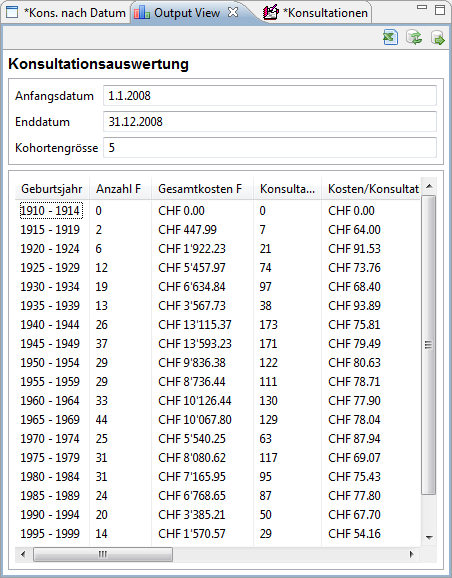
\includegraphics{kohorte}\\
  \caption{Auswertung je Kohortengrösse}\label{Abb1}
\end{figure}

\begin{figure}
  % Requires \usepackage{graphicx}
  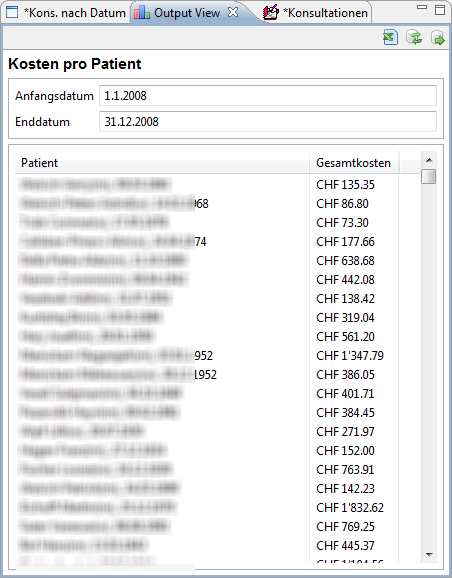
\includegraphics{patient}\\
  \caption{Auswertung nach Patienten}\label{Abb2}
\end{figure}

\end{document} 